% !TeX root = ../libro.tex
% !TeX encoding = utf8
%
%*******************************************************
% Métricas
%*******************************************************

\chapter{Métricas}\label{ch:metricas}

Enumeramos y explicamos distintas \textbf{métricas}: funciones que nos sirven para medir la bondad del ajuste de los modelos en distintos problemas. Es importante no confundir la métrica usada para medir el rendimiento de los modelos, con la función de error o pérdida que usa cada modelo concreto y trata de minimizar, ya que se puede minimizar distintas funciones de error pero que impliquen un buen resultado en la métrica; aun así es posible que coincida la métrica con la función de error.

Según la tipología del problema podemos encontrar distintas métricas donde veremos las más importantes de los problemas de clasificación y regresión.

\section{Clasificación}

En los problemas de clasificación nos encontramos con aprendizaje \textbf{supervisado} ya que generalmente tenemos unas etiquetas ascoiadas a los datos que queremos predecir correctamente. Según el modelo puede tener dos tipos de enfoque para los que tendremos distintos tipos de métricas: predicción de etiquetas (clasificador "duro") o predicción de probabilidades asociadas a las clases (clasificador "flexible").

Planteamos antes el problema general de clasificación con $n$ clases con la siguiente definición

\begin{definicion}[Problema de clasificación multiclase]
  Sea $M \in \N$ la longitud de las series, $N \in \N$ el número de series y $n$ el número de clases, se considera el espacio $\mathcal{X} \times Y \subseteq \R^M \times \{0, 1, \ldots, n - 1\}$ del que se extrae una muestra $(X, \textbf{y}) \in \mathcal{X}^N \times Y^N$ que sigue una distribución $\mathcal{P}$ desconocida y el espacio de funciones del modelo dado $\mathcal{H}$.

  El problema consiste en encontrar un $h \in \mathcal{H}$ de tal manera que $h \approx f$, siendo $f$ la función de etiquetado:
  \begin{align*}
    f : \mathcal{X} & \to Y \\
    \textbf{x} & \mapsto f(\textbf{x}) \in \{0, 1, 2, \ldots, n - 1\}.
  \end{align*}
  \label{def:clasgen}
\end{definicion}

Como nota, en los problemas de clasificación binarios se suele indicar una clase como la positiva ($+1$) y la otra como la negativa ($-1$); normalmente la positiva es la que tiene más relevancia para ser detectada que la negativa, aunque no tiene por qué. Ademas, en clasificación multiclase se puede considerar la clase más importante, si la hubiera, como la positiva y el resto la negativa; o también considerar para cada clase como si fuese la positiva y tomar la media de todos los resultados.

\subsection{Etiquetas}

Si nuestro clasificador devuelve etiquetas, suponiendo que la muestra tiene las clases balanceadas y que importan lo mismo, la métrica más usada es el acierto (\emph{accuracy}) que mide simplemente la proporción de correspondencia de las etiquetas predichas con las originales.

Dada la función aprendida por un modelo $h \in \mathcal{H}$, definimos $acc$ como
\begin{equation*}
  acc(h) = \frac{1}{n} \sum \limits^N_{i = 1}[[h(\textbf{x}_i) = y_i]].
  \label{eq:acc}
\end{equation*}

Considerando que $acc \in [0, 1]$ se puede también usar la función de pérdida asociada como
\begin{equation*}
  E(h) = 1 - acc(h),
  \label{eq:acc_loss}
\end{equation*}
aunque es más frecuente usar $acc$.

Cuando la clase positiva importa más que la negativa tenemos que medir de otra manera para tener en cuenta que una clase influye más que la otra. Para ello introducimos los los conceptos de \textbf{precisión} ($precision$) y \textbf{sensibilidad} ($recall$):

\begin{enumerate}
  \item \textbf{Precisión}: definido como
    \begin{equation*}
      precision = \dfrac{verdaderos\_positivos}{verdaderos\_positivos + falsos\_positivos},
      \label{eq:precision}
    \end{equation*}
    evalúa la proporción de las clases positivas correctamente clasificadas frente a todas las etiquetadas como la clase positiva. Si el modelo es muy preciso nos indica que cuando el modelo etiqueta un dato con la clase positiva casi seguro que lo sea.
  \item \textbf{Sensibilidad}: definido como
  \begin{equation*}
    recall = \dfrac{verdaderos\_positivos}{verdaderos\_positivos + falsos\_negativos},
    \label{eq:recall}
  \end{equation*}
  evalúa la proporción de las clases positivas correctamente clasificadas frente a todas las clases positivas que hay, bien o mal clasificadas. Si el modelo es muy sensibile nos indica que clasifica correctamente la mayoría de datos con etiqueta positiva.
\end{enumerate}

Usando estos dos valores se define la métrica $F_\beta$
\begin{equation}
  F_\beta = (1 + \beta^2) \cdot \dfrac{precision \cdot recall}{(\beta^2 \cdot precision) + recall},
  \label{eq:fscore}
\end{equation}
donde variamos el $\beta$ usado según la matriz de costes asociados a los falsos positivos y negativos. Generalmente se usa $F_1$ cuando cuestan igual, $F_{0.5}$ si los falsos positivos cuestan más y $F_{2}$ si son los falsos negativos los que más cuestan.

\subsection{Probabilidades}

Aunque el clasificador devuelve probabilidades generalmente necesitamos dar una respuesta con etiquetas, por lo que se suele dar un \textbf{umbral} para el que clasificar como una clase (problema binario) o tomar la clase con mayor probabilidad si se están prediciendo probabilidades para todas las clases.

En cualquier caso las dos métricas más usadas generalmente son las que miden el \textbf{área bajo la curva} de las funciones \textbf{precision-recall} ($PR-AUC$) y \textbf{Receiver Operating Characteristic} ($ROC-AUC$). En ambos casos se crea una curva en el cuadradado $[0,1] \times [0,1]$ donde se integra para obtener el área que deja la curva, haciendo que ambas métricas tomen valores en $[0, 1]$ siendo mejor el modelo cuanto más alto valga.

Cuando la clase positiva importa igual que la clase negativa se toma $ROC-AUC$ que mide el comportamiento del modelo obteniendo las tasas de falsos positivos ($falsos\_positivos$) y verdaderos positivos ($verdaderos\_positivos$) para cada umbral de probabilidad que se va poniendo al modelo. Se suele imprimir el gráfico con la curva que forma comparando con el clasificador aleatorio para compararlo (\autoref{fig:ej-roc} \cite{scikit2020roc}).

\begin{figure}[htpb]
  \centering
  %\hspace*{-2.5cm}
  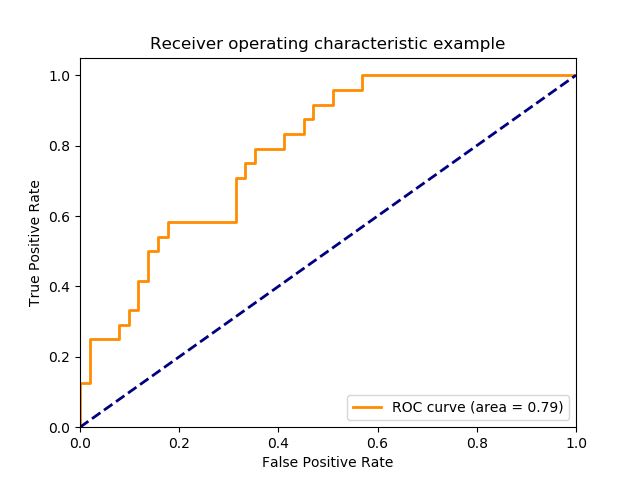
\includegraphics[width=.6\textwidth]{ej-roc}
  \caption{Ejemplo de curva ROC.}
  \label{fig:ej-roc}
\end{figure}

Por otro lado, si la clase positiva tiene mayor importancia entonces se coge $PR-AUC$ que en este caso mide la precisión y la sensibilidad del modelo frente a distintos umbrales de probabilidad. También se incluye un modelo aleatorio para hacer la comparación, donde encontramos un ejemplo en \autoref{fig:ej-pr} \cite{scikit2020pr}.

\begin{figure}[htpb]
  \centering
  %\hspace*{-2.5cm}
  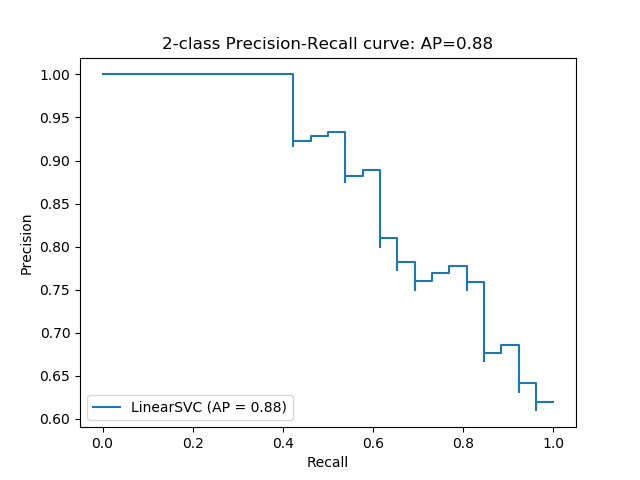
\includegraphics[width=.6\textwidth]{ej-pr}
  \caption{Ejemplo de curva PR.}
  \label{fig:ej-pr}
\end{figure}

\section{Regresión}

Un problema de regresión no es más que un problema de clasificación donde las etiquetas no son discretas sino continuas (\autoref{def:probregresion}).

\begin{definicion}[Problema de regresión]
  Sea $M \in \N$ la longitud de las series y $N \in \N$ el número de series y $n$ la dimensión de las etiquetas, se considera el espacio $\mathcal{X} \times \mathcal{Y} \subseteq \R^M \times \R^n$ del que se extrae una muestra $(X, Y) \in \mathcal{X}^N \times \mathcal{Y}^N$ que sigue una distribución $\mathcal{P}$ desconocida y el espacio de funciones del modelo dado $\mathcal{H}$.

  El problema consiste en encontrar un $h \in \mathcal{H}$ de tal manera que $h \approx f$, siendo $f$ la función de etiquetado:
  \begin{align*}
    f : \mathcal{X} & \to \mathcal{Y} \\
    \textbf{x} & \mapsto f(\textbf{x}) \in \R^n.
  \end{align*}
  \label{def:probregresion}
\end{definicion}

Generalmente se usan las siguientes métricas principales, donde todas toman valores en $[0, +\infty)$ siendo cuanto más bajo mejor:

\begin{enumerate}
  \item \textbf{Error Medio Absoluto} (\emph{Mean Absolute Error}, MAE): definido como
  \begin{equation*}
    MAE(h) = \dfrac{1}{n} \sum \limits^N_{i = 1} || \textbf{y}_i - h(\textbf{x}_i) ||_1,
    \label{eq:mae}
  \end{equation*}
  se suele usar para no tener en cuenta el efecto de los valores atípicos ya que es menos sensible a estos.
  \item \textbf{Error Cuadrático Medio} (\emph{Mean Squared Error}, MSE): definido como
  \begin{equation}
    MSE(h) = \dfrac{1}{n} \sum \limits^N_{i = 1} || \textbf{y}_i - h(\textbf{x}_i)) ||^2_2,
    \label{eq:mse}
  \end{equation}
  es una de las métricas mayormente usadas y añade importancia a errores grandes, ya que se aplica un cuadrado.
  \item \textbf{Raíz del Error Cuadrático Medio} (\emph{Root Mean Squared Error}, RMSE): definido como
  \begin{equation*}
    RMSE(h) = \sqrt{MSE(h)}.
    \label{eq:rmse}
  \end{equation*}
  hace que las medidas del MSE vuelvan a la unidad, dando una mejor interpretabilidad.
\end{enumerate}

\endinput
